\chapter[Hyperdimensional computing]{Hyperdimensional Computing}
\section{Introduction}
Hyperdimensional computing (HDC) is a relatively recent paradigm of computing in which data is represented and manipulated by high-dimensional (or hyperdimensional) vectors in the range of tens of thousands bits. This framework, outlined by Kanerva~\cite{Kanerva2009}, is inspired by the workings of the human brain and its ability to adapt, learn fast and easily understand semantic relations. The human brain consists of about 100 billion neurons (nerve cells) and 1000 trillion synapses that connect these neurons. Each neuron is connected to up to 10,000 other neurons, creating massive circuits. This is likely fundamental to the workings of the human brain and what distinguishes our brains from modern von Neumann computer architectures, which operate on 8 to 64-bit vectors. This becomes clear when we compare the relative simplicity for a human to learn a language compared to computers. Computers use a large and complicated set of arithmetic operations in the form of deep learning networks, which require terabytes of data and thousands of Watts of computing power to come close to mastering a language whilst a human can recognize other languages relatively easily when they don't even speak it. Likewise languages, we can very easily memorize and compare other intrinsically complex and contextual concepts such as images. A computer would have a hard time finding similarities between a set of images and faces because this requires very complex machine learning models. The human brain can do this all with a very large efficiency by consuming only roughly 20 W of energy.

Achieving these kinds of flexible brain-like models based on high dimensionality is not entirely new and is being explored since the 1990s. Some of these earlier models include Holographic Reduced Representations~\cite{HRR}, Spatter Code~\cite{spatter} and others. A hyperdimensional vector (HDV) can represent anything from a scalar number to any kind of concept. This vector is initially made up of totally random elements, but with a simple set of operations, which will be explained later, we can use other vectors to combine some concepts into new similar or dissimilar concepts. For example, to show the essence of HDC and how it tries to simulate the brain, we can compare the concept of a \textit{table} to the concept of a \textit{brocolli}. We would not immediately conclude that they are in any way similar but as humans, we can trace back \textit{table} to \textit{plate}, which has some similarities with \textit{food} from which we can easily extract the concept of \textit{brocolli} as in Eq. \ref{eqn:sem}. These kinds of operations are not very obvious for a classical computer but creating these semantic pathways and recognizing links between distant objects are rather easy for humans. Two unrelated concepts are noted by $\neq$ and two related concepts by $\approx$.
\begin{align}\label{eqn:sem}
    \begin{split}
    &\textrm{table} \neq \textrm{brocolli} \\        
    &\textrm{table} \approx \textrm{plate} \approx \textrm{food} \approx \textrm{brocolli}
    \end{split}
\end{align}
The elements in an HDV can be made up of binary bits (values from the set \{0, 1\}) like in classical computing but also of bipolar (values from the set \{-1, 1\}) or real numbers. The choice of the nature of the elements has also implications on the nature of the different operations and possibly the results.

An initial HDV is generated randomly. This \textit{holistic} or \textit{holographic} representation of a concept spread out over a vector consisting of thousands of bits gives rise to interesting properties such as its robustness against noise~\cite{hdctheo}. These kinds of systems are also very tolerant to failure of bits since we introduce a lot of redundancy in the vector just by stochasticity. This is very unlike classical computing where every bit counts and one failure in a bit can lead to immediate data corruption. Besides its robustness, it also has the potential to perform much faster and more efficient computations than traditional computer systems since it allows for more efficient data storage by encoding multiple objects into a vector~\cite{Kanerva2009}\cite{hdctheo}.
\section{Operations on hyperdimensional vectors}
The interesting properties of HDC are based on only four basic operations we can perform on HDVs. We will discuss these for bipolar and binary vectors. From here, all implementations are written in the programming language Julia~\cite{Julia} unless noted otherwise. Known for its efficiency, Julia's blend of high-level, interpreter-based features makes it possible to write powerful programs. This is particularly beneficial when working with high-dimensional spaces. Julia's built-in support for bitvectors and bitmatrices, along with parallel computing, will be useful for this thesis. Furthermore, the lively Julia community supports a rich ecosystem and a broad array of packages to utilize.

Before the operations are demonstrated, we show how a random hyperdimensional vector can be generated in Julia. In the following code block, functions to generate binary and vectors can be made effortlessly with one line each.

\begin{minted}{julia}
# Built-in package for random number generation
using Random

# Binary HDV
bithdv(N::Int=10_000) = bitrand(N) 
#Bipolar HDV
hdv(N::Int=10_000) = rand((-1,1), N)
\end{minted}

\subsection*{Bundling} \label{sssec:add}
Also referred to as \textit{superposition} or \textit{aggregation}, the element-wise addition as in Eq.~\ref{eqn:sum} of $n$ input vectors $[X_{1} + X_{2} + \cdots + X_{n}]$ creates a vector $X$ that is similar to the input vectors.
\begin{equation}
    \label{eqn:sum}
    X = [X_{1} + X_{2} + \cdots + X_{n}]\,.
\end{equation}
For bipolar vectors, this entails a straightforward element-wise addition. The resulting vector is restricted to a bipolar nature too depending on the sign of each element, thus containing only $-1$, $1$ but allowing $0$ for elements that are in disagreement as shown in the following $6$-dimensional example.
\begin{alignat*}{7}
    X_{1} &= && \qquad +1 && \qquad -1 && \qquad +1 && \qquad +1 && \qquad -1 && \qquad -1 \\
    X_{2} &= && \qquad +1 && \qquad +1 && \qquad +1 && \qquad -1 && \qquad -1 && \qquad -1 \\
    X_{3} &= && \qquad -1 && \qquad -1 && \qquad +1 && \qquad +1 && \qquad -1 && \qquad +1 \\
    X_{4} &= && \qquad -1 && \qquad -1 && \qquad -1 && \qquad +1 && \qquad -1 && \qquad +1 \\
    \hline
    [X_{1} + X_{2} + X_{3} + X_{4}] &= && \qquad \phantom{-}0 && \qquad -1 && \qquad +1 && \qquad +1 && \qquad -1 && \qquad \phantom{-}0
\end{alignat*}

For binary vectors, the vectors are element-wise bundled based on the majority element. This is no problem if an odd number of input vectors are considered but ambiguity arises when bundling an even set of vectors. This can be solved by setting the element in question randomly~\cite{binBund}. Another possibility is to add another random vector however this may seem to add more unnecessary noise, especially when bundling a low number of vectors. We can also reverse the bundling operation using an \textit{inverse addition}. For bipolar vectors, this would involve multiplying the vector of interest by -1. A binary vector can be flipped bit-wise. While these types of operations are not directly built into Julia, they can be easily programmed as follows:

\begin{minted}{julia}
# Adds bitvectors element-wise based on the majority element.
# Random if tied.
# Reduce function takes another function (here .+)
# and applies it to all given vectors.
# 'Dotted' operations such as .+ are vectorized
# making it element-wise.
function bitadd(vectors::BitVector ...)
    v = reduce(.+, vectors)            
    n = length(vectors) / 2
    x = [i > n ? 1 : i < n ? 0 : rand(Bool) for i in v]
    return x
end

# Adds bipolar vectors element-wise and rounds off to -1,0 or 1
# depending on the resulting sign.
add(vectors...) = reduce(.+, vectors) .|> sign
\end{minted}
Similar to an ordinary arithmetic summation, the bundling addition of hyperdimensional vectors is commutative so the result is not dependent on the order of addition.
\begin{equation}
    \label{eqn:sumcom}
    [X_{1} + X_{2}] = X = [X_{2} + X_{1}]\,.
\end{equation}
\subsection*{Binding} \label{sssec:mult}
Two vectors can be multiplied element-wise resulting in a vector maximally dissimilar to the input vectors. Vectors $X$ and $Y$ are bound together forming $Z$ being orthogonal to $X$ and $Y$ as shown in Eq.~\ref{eqn:multp}.
\begin{equation}
    \label{eqn:multp}
    Z = X \circ Y\,.
\end{equation}
This \textit{binding} operation translates to a simple arithmetic element-wise multiplication for bipolar vectors. For binary vectors, it is represented by a \textit{XOR} bit-operation shown as follows:
\begin{alignat*}{7}
    X &= && \qquad 1 && \qquad 0 && \qquad 1 && \qquad 1 && \qquad 0 && \qquad 0 \\
    Y &= && \qquad 1 && \qquad 1 && \qquad 0 && \qquad 1 && \qquad 0 && \qquad 1 \\
    \hline
    X \circ Y &= && \qquad 0 && \qquad 1 && \qquad 1 &&  \qquad 0 && \qquad 0 && \qquad 1
\end{alignat*}
In Julia, there is a built-in function to carry out bit-operations such as \textit{XOR}. For bipolar vectors, a simple element-wise multiplication suffices.

\begin{minted}{julia}
# Bind binary vectors
bitbind(vectors::BitVector ...) =  reduce(.xor, vectors)

# Bind bipolar vectors
bind(vectors...) = reduce(.*, vectors)
\end{minted}

The binding operation can also be undone by multiplying with the same vector again. It is its own inverse so that:
\begin{equation}
    \label{eqn:multpinv}
    A \circ A = O\,,
\end{equation}
where $O$ is a vector containing only zeros. Like an ordinary multiplication, this operation is commutative and distributive over addition, meaning that transforming a bundle of concepts with binding is equivalent to binding every element before bundling:
\begin{equation}
    \label{eqn:multpdis}
    A = Z \circ (X + Y) = X \circ Z + Y \circ\ Z\,.
\end{equation}
\subsection*{Permutation} \label{sssec:perm}
The permutation operation of an HDV is a reordering of the contents of the HDV. This can be random but a circular shift is widely employed~\cite{HD_rev} and makes the operation easily reversible. It results in a vector technically dissimilar from the input vector but still encoding its information. This property will become important later when it will be used to encode sequential information such as tokens in a text. This operation will be denoted by $\Pi$.
\begin{alignat*}{7}
    X &= && \qquad 1 && \qquad 0 && \qquad 1 && \qquad 1 && \qquad 0 && \qquad 0 \\
    \hline
    \Pi(X) &= && \qquad 0 && \qquad 1 && \qquad 0 &&  \qquad 1 && \qquad 1 && \qquad 0
\end{alignat*}
In Julia, this line can do it for both binary and bipolar vectors:

\begin{minted}{julia}
# Permute by applying a circular shift
perm(vector::AbstractVector, k::Int=1) = circshift(vector, k)
\end{minted}

\subsection*{Similarity measurement} \label{sssec:sim}
For many kinds of problems, it will be necessary to quantify the similarity between two HDVs. The method depends on the nature of the vectors. For binary vectors, the \textit{Hamming distance} defined as:

\begin{equation}
    \label{eqn:Hamming}
    \text{Ham}(A, B) = \frac{1}{d} \sum_{i=1}^{d} 1_{A_{(i)} \neq B_{(i)}}
\end{equation}
The \textit{cosine distance} as defined in Eq.~\ref{eqn:cosine} is most commonly used for bipolar vectors:
\begin{equation}
    \label{eqn:cosine}
    S_{C}(A, B) = \frac{A \cdot B}{||A|| * ||B||}
\end{equation}
Both are not built-in Julia by default, but can be programmed as follows:
\begin{minted}{julia}
# Built-in package for linear algebra operations 
using LinearAlgebra

# Hamming distance
hamming(x::BitVector, y::BitVector) = sum(x .!= y)/length(x)

# Cosine similarity
cosine(x::Vector, y::Vector) = dot(x, y) / (norm(x) * norm(y))
\end{minted}
The results of both of these measurements are summarized in Table~\ref{tab:dist}.
\begin{table}[h]
    \centering
    \caption{\label{tab:dist}Overview of similarity measurements in HDC depending on the nature of the HDVs}
    \begin{tabular}{|cccc|}
        \hline
        \textbf{Measurement} & \textbf{Dissimilar} & \textbf{Orthogonal} & \textbf{Similar} \\
        \hline
        \textbf{Hamming distance} & 1 & 0.5 & 0 \\
        \hline
        \textbf{Cosine similarity} & -1 & 0 & 1 \\
        \hline
    \end{tabular} 
\end{table}

It is important to note that two random HDVs will be quasi-orthogonal to each other just by stochasticity. Also note that the first quantifies a distance and the latter a similarity.
\section{Demonstration of hyperdimensional computing on simple examples}
There are many interesting possibilities given the relative simplicity of all these operations. In this section, we will demonstrate the power of hyperdimensional computing with some simple examples.
\subsection*{Simple example with simulated data}
To get a feel for the operations, assume $A, B, C, X, Y$ and $Z$ to be random 10,000-dimensional bipolar hypervectors and that $D = X \circ A + Y \circ B + Z \circ C$, let us then try to retrieve $A$ from $D$ by using the defined operations. We generate for each of $A, B, C, X, Y$ and $Z$ a random 10,000-D vector. To retrieve an approximation of $A, D$ can be multiplied by $X$ and the rest of the included vectors are then regarded as noise as done in Eq.~\ref{eqn:ex1}. Because of the robustness of hyperdimensional vectors, a lot of information of $A$ should still be contained within $D$.
\begin{align}\label{eqn:ex1}
\begin{split}
    A' &= X \circ D \\
    &= X \circ (X \circ A + Y \circ B + Z \circ C) \\
    &= \underbrace{X \circ X \circ A}_A + \underbrace{X \circ Y \circ B + X \circ Z \circ C}_\text{noise} \\
    &\approx A
\end{split}
\end{align}
 The procedure of Eq.~\ref{eqn:ex1} is repeated 10,000 times because of the stochastic nature of these vectors. The results are illustrated in Figure~\ref{fig:exm1}.
\begin{figure}[h]
    \centering
    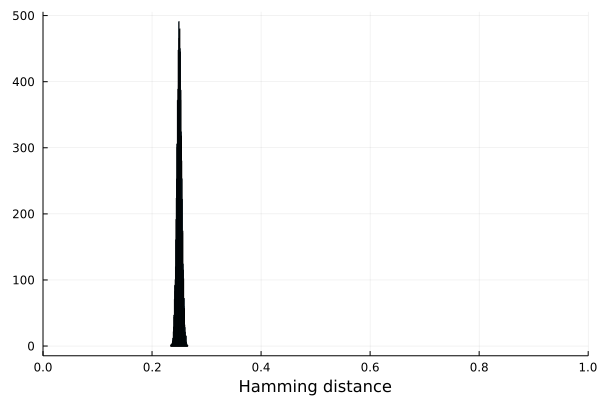
\includegraphics[scale = 0.2]{output.png}
    \caption{10,000 cases of random 10,000-dimensional binary vectors being made by Eq.~\ref{eqn:ex1}. The resulting Hamming distances between $A$ and $A'$ are then plotted in a histogram. The dashed line indicates a Hamming distance of 0.5, meaning that two vectors are orthogonal.}
    \label{fig:exm1}
\end{figure}
We see that we can retrieve a lot of information with most of the Hamming distances centering around 0.25. Due to the high-dimensional space and thus its robustness, the distances are very consistent. Note that two completely random HDVs would have a distance close to 1 just by stochasticity. A Hamming distance of 0 would mean that we retrieved all bits of A correctly, which is impossible in this model due to the consideration of noise. Although we work with a very constrained model, vector $A$ is roughly 75 \% retrievable and the calculations are very efficient as all of these can be completed in less than 2 seconds on a laptop. This same experiment was done with random bipolar, 10,000-dimensional vectors and it performs slightly slower as expected but retained the accuracy.
\subsection*{Examples of hyperdimensional computing on real datasets}
\label{sec:example}
Now, the power of these simple operations will be demonstrated by applying them to a couple of relatively small real datasets.
\subsection*{Zoo animal classification}
As the first example, we will consider a simple dataset containing 101 animals with 17 descriptors such as their number of legs, their skin covering and other physical properties~\cite{zoo}. Our goal is to create a simple model that can classify these animals and other animals that are not present in the dataset based on their descriptors. To tackle this problem, we first assign to each descriptor a random hyperdimensional vector. For each animal, all of its features can be bundled to obtain a final vector representing the animal. For example, it is known that a chicken lays eggs, is covered with feathers and has two legs so then these features can be bundled as in the following equation. $C$ is a vector representing a chicken, $E$ the ability to lay eggs, $F$ the possession of feathers and $T$ the possession two legs:
\begin{equation}\label{eqn:chicken}
    C = E + F + T\,.
\end{equation}
This is simple for all the variables that have binary values, but the feature for the number of legs is variable. Although it is possible to assign completely random vectors to each number of legs, it would make a slightly more biologically realistic model if an animal with 2 legs would be more similar to one with 4 legs than to one with 8 legs. To address this, a range of numbers would have to be representable by hyperdimensional vectors, the range from 0 to 8 in this case. First, a random hyperdimensional vector representing the lower bound of the interval is generated. Next, a vector representing the next step in the interval is constructed by replacing a fraction of the vector with random bits. This last step is then repeated to obtain a vector of each number in a range.

In biology, it is possible to find higher-order of concepts that are combinations of directly observable characteristics. For example, an animal could lay eggs or be dependent on its mother's milk, but (almost) never both. So, the growth and development of an animal depend on these characteristics. This property can be easily implemented into this HDC model by binding an HDV of a higher order concept to the descriptor HDV. So as said previously, the 'milk' ($M$), and 'egg' ($E$) features yields information about the growth of the animal, so we will create another vector representing the growth feature ($G$) to obtain a more expanded model. This is also done for the skin protection features ($S$) and all the features considering the limbs ($L$). This also gives us the possibility to retrieve some features of the animals as in the procedure shown in the previous example. Thus, Eq.~\ref{eqn:chicken} can be expanded into:
\begin{equation}
    C = G \circ E + S \circ F + L \circ T\,.
\end{equation}

After conducting the various procedures, the data set now consists of 101 animals, each represented by a 10,000-dimensional feature vector. To efficiently analyze and visualize this high-dimensional data, principal component analysis (PCA) has been employed to reduce the dimensionality from 10,000 to just two. By projecting these vectors onto a 2D space, the data can be conveniently displayed in a two-dimensional plot, as illustrated in Figure \ref{fig:exm2}. Upon examination of the plot, three distinct and meaningful clusters of animal classes emerge, which align well with our understanding of evolutionary relationships. These clusters include: (1) mammals, (2) a group consisting of birds, reptiles, and amphibians, and (3) a cluster encompassing invertebrates and insects. While the current analysis already provides valuable insights into the relationships between different animal classes, further improvement could be achieved by incorporating additional features that may lead to a clearer separation of these groups. By doing so, the model would be able to more accurately distinguish between the different animal classes and provide a more comprehensive understanding of their evolutionary connections.
\begin{figure}[h]
    \centering
    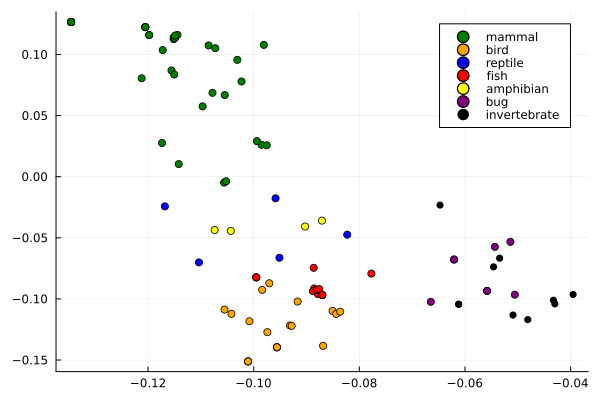
\includegraphics[scale = 0.5]{pca1.png}
    \caption{Scatter plot of the first two principal components (PCs) of a 101$\times$10,000 matrix containing hyperdimensional vectors for every animal in the zoo dataset after a PCA procedure. These PCs account for roughly 48 \% of the variance.}
    \label{fig:exm2}
\end{figure}

After an HDV has been made for every animal, all animals of the same class can be bundled to obtain an HDV representing the said class. So for example, if we have a hyperdimensional vector for a pigeon ($P$), chicken ($C$) and a kiwi ($K$), an HDV representing birds ($B$) can be made by doing:
\begin{equation}
    B = [P + C + K]\,.
\end{equation} 
To classify an animal, its HDV can be compared to the HDVs of every class and the most similar vector is then assumed to be its class.  In the following code block, the hypervectors for every animal and class have been already made as discussed above. The resulting HDV for a flamingo has been compared to every other class vector \textit{via} a measurement of the Hamming distance. The distance of flamingo HDV to the bird HDV is significantly smaller than to all other vectors
\begin{figure}[H]
    \centering
\begin{minted}{julia}
# HDVs for every animal class HDVs have been made already
# Take flamingo HDV out of dataframe
flamingo = data.species_hdv[24]
println("Hamming distance to mammal = ",
hamming(flamingo, mammal))

println("Hamming distance to bird = ",
hamming(flamingo, bird))

println("Hamming distance to reptile = ",
hamming(flamingo, reptile))

println("Hamming distance to amphibian = ",
hamming(flamingo, amphibian))

println("Hamming distance to bug = ",
hamming(flamingo, bug))

println("Hamming distance to fish = ",
hamming(flamingo, fish))

println("Hamming distance to invertebrate = ",
hamming(flamingo, invertebrate))

# Output
# Hamming distance to mammal = 0.303
# Hamming distance to bird = 0.1044
# Hamming distance to reptile = 0.2727
# Hamming distance to amphibian = 0.313
# Hamming distance to bug = 0.2867
# Hamming distance to fish = 0.3484
# Hamming distance to invertebrate = 0.4061
\end{minted}
\end{figure}
For further improvement, it would be possible to generate a set of animals not present in the dataset and test those in order to further understand how this model can be improved. On top of this, it would also be possible to generate a confusion matrix to understand where we could use more distinguishing descriptors. From the PCA, we could already predict that reptiles and amphibians would be easily confused, as for invertebrates and bugs.
\subsection*{Protein classification}
\label{ssec:protclas}
To illustrate an example more akin to this research topic, a model based on the principles of hyperdimensional computing will be built to classify a protein sequence dataset~\cite{anticancer}. It contains 949 manually curated peptide sequences with their membranolytic anti-breast cancer activity level (very active, moderately active, experimentally inactive and virtually inactive). The virtually inactive peptides are predicted to be inactive. The model will be built with mostly the same procedure as for the animal classifier, but instead of animals, sequences have to be encoded into HDVs now. First, a random HDV is generated for every amino acid. Physicochemical properties, evolutionary constraints etc. could be introduced to make this model more realistic but that is not necessary for this demonstration. Next, a peptide sequence is to be considered as a bag of trimers as seen in Figure~\ref{fig:diagram_exprot5}. A vector representing a trimer is generated by binding the three amino acids whilst retaining sequential information by shifting as in Eq.~\ref{eqn:trimer}. All retrievable trimers from a given sequence are then bundled together, forming a vector representative of the sequence. 
\begin{equation}\label{eqn:trimer}
    ABC = A \circ \Pi (B) \circ \Pi (\Pi (C))\,.
\end{equation}
\begin{figure}[h!]
    \centering
    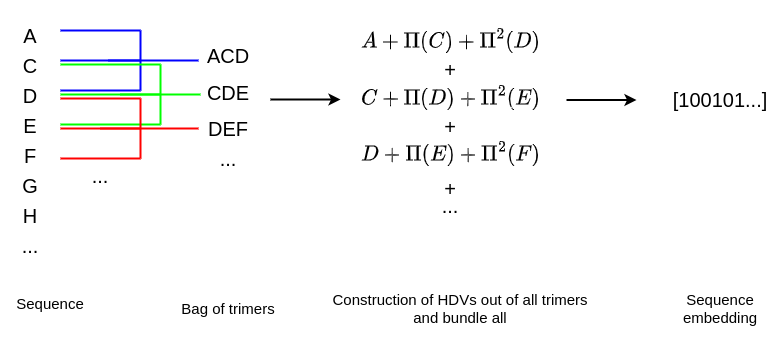
\includegraphics[scale = 0.55]{diagram_exprot.png}
    \caption{Overview of operations done to obtain an HDV of a protein sequence for the example concerning the real peptide dataset. First, a random HDV is generated for every amino acid. Next, a peptide sequence is to be considered as a bag of trimers. A vector representing a trimer is generated by binding the three amino acids whilst retaining sequential information by shifting as in Eq.~\ref{eqn:trimer}. All retrievable trimers from a given sequence are then bundled together, forming a hyperdimensional vector representation of the sequence.}
    \label{fig:diagram_exprot5}
\end{figure}
From here on, the same procedures as in the last example can be applied here too, so all HDVs of a class are bundled for further analysis. The PCA procedure did not generate interesting results because the two first principal components explained only 5 \% of the variance. This means that it is not feasible to reduce the 10,000 dimensions of the vectors to two, likely because the information is too smeared out over the vectors. This occurrence is highly dependent on the training data. Nevertheless, this follows the philosophy of hyperdimensional computing in keeping holistic representations of concepts.

\begin{figure}[h!]
    \centering
    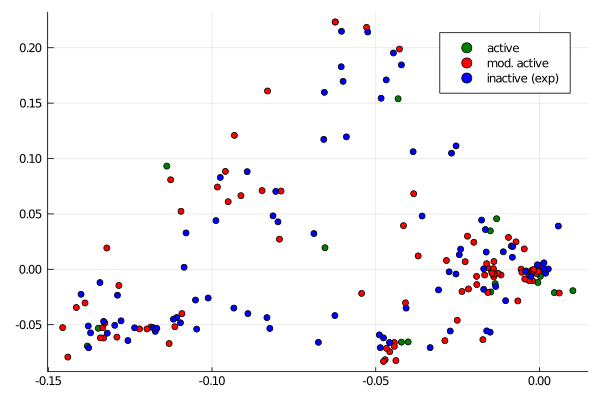
\includegraphics[scale = 0.5]{exampprot.png}
    \caption{Scatter-plot of the first two principal components, projecting the 10,000-dimensional vectors for every peptide into the two main PCs. These PCs account for roughly 5 \% of the total variance}
    \label{fig:diagram_exprot}
\end{figure}

Next, a classifier was made correspondingly. The dataset was stratified and split into a training set (comprising 80 \% of the sequences) and a test set. With 100 runs, it could predict a protein sequence's class with an accuracy of 85 \%. It has to be taken into account that the predicted inactive peptides account for 80 \% of the sequences of the dataset, thus this model performs slightly better than if we would predict at random given the sample balances. There are many possible improvements to be made however, such as using more suitable performance metrics, introducing similarities between amino acids instead of setting them randomly and using more suitable frameworks for our protein classification models, which will all be research topics further on in this project.